% !TeX program = xelatex
% !TeX encoding = UTF-8
% !TeX root = main.tex
% 在本文件所在目录运行：latexmk main.tex
\documentclass[UTF8,fontset=fandol,a4paper,zihao=-4,oneside,openany]{ctexbook}
\usepackage{config/note-style}

% ---------- 只需先修改以下信息 ----------
\newcommand{\NoteTitle}{论文或学习笔记标题}
\newcommand{\NoteSubtitle}{通用写作模板}
\newcommand{\NoteAuthor}{作者姓名}
\newcommand{\NoteInstitution}{学校或单位名称}
\newcommand{\NoteCourse}{专业或课程名称}
\newcommand{\NoteAdvisor}{指导教师姓名}
\newcommand{\NoteDate}{\today}

% 没有引文时可改为 \notebibliographyfalse。
\newif\ifnotebibliography
\notebibliographytrue
\hypersetup{pdftitle={\NoteTitle},pdfauthor={\NoteAuthor}}

\begin{document}
\frontmatter
\makenotetitle
% !TeX root = ../../main.tex
\chapter*{摘要}
\addcontentsline{toc}{chapter}{摘要}
此处简述研究目的、方法与主要结论。

\par\noindent\textbf{关键词：}关键词一；关键词二；关键词三

\chapter*{Abstract}
\addcontentsline{toc}{chapter}{Abstract}
Replace this paragraph with the purpose, method, and main findings.

\par\noindent\textbf{Keywords:} keyword one; keyword two; keyword three

\tableofcontents
\mainmatter

% 正文：七章框架。按需修改标题、增删文件，并同步调整载入列表。
% !TeX root = ../../main.tex
% 结构来源：原笔记第 1 个正文文件的任务与目标梳理。
\chapter{绪论}
\label{chap:introduction}

\section{研究背景}
此处填写研究背景。文献引用示例见\cite{lamport1994latex}。

\section{研究目标与内容}
此处填写研究目标和主要任务。

\section{章节安排}
此处简述各章内容。

% !TeX root = ../../main.tex
% 结构来源：原笔记第 2 个正文文件的基础概念与方程。
\chapter{基础理论}
\label{chap:theory}

\section{基本概念}
此处介绍基本概念。
\begin{definition}[向量]
\(\dimvec{x}{3}\) 表示三维列向量。
\end{definition}

\section{符号约定}
常用符号见附录\ref{app:symbols}。

% !TeX root = ../../main.tex
% 结构来源：原笔记第 3 个正文文件的模型假设与状态关系。
\chapter{模型建立}
\label{chap:model}

\section{模型假设}
此处填写模型假设与适用范围。

\section{模型表达}
以下仅演示矩阵公式的排版：
\begin{equation}
  \dimmat{A}{3}{3}\dimvec{x}{3}=\dimvec{b}{3}.
  \label{eq:linear-model}
\end{equation}

\subsection{条件说明}
此处填写初始条件或边界条件。

% !TeX root = ../../main.tex
% 结构来源：原笔记第 4 个正文文件的模型比较与方法展开。
\chapter{方法与推导}
\label{chap:method}

\section{研究方法}
此处说明研究方法。

\section{推导示例}
\begin{theorem}
若矩阵 \(A\) 可逆，则方程 \(Ax=b\) 的解为 \(x=A^{-1}b\)。
\end{theorem}
\begin{proof}
在等式两侧左乘 \(A^{-1}\) 即得。
\end{proof}

较长的计算可移至附录\ref{app:derivation}。

% !TeX root = ../../main.tex
% 结构来源：原笔记第 5 个正文文件的关键关系与结果整理。
\chapter{结果与分析}
\label{chap:results}

\section{结果展示}
表\ref{tab:example}与图\ref{fig:example}仅为排版示例。
\begin{table}[htbp]
  \centering
  \caption{示例数据}\label{tab:example}
  \begin{tabular}{ccc}
    \toprule
    序号 & 输入 & 输出 \\
    \midrule
    1 & 1 & 2 \\
    2 & 2 & 4 \\
    3 & 3 & 6 \\
    \bottomrule
  \end{tabular}
\end{table}

\begin{figure}[htbp]
  \centering
  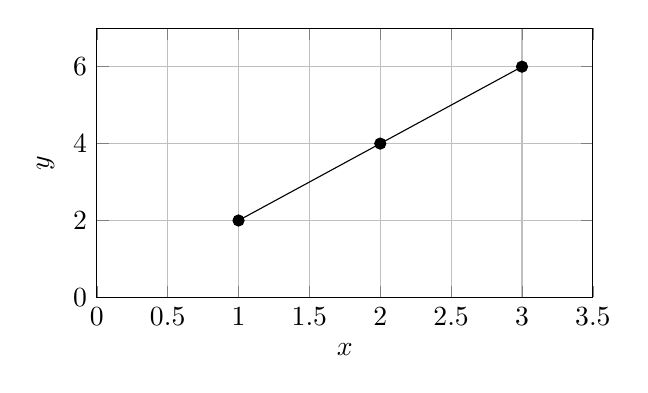
\begin{tikzpicture}
    \begin{axis}[
      width=0.65\linewidth,height=5cm,
      xlabel={$x$},ylabel={$y$},
      xmin=0,xmax=3.5,ymin=0,ymax=7,
      grid=major
    ]
      \addplot[black,mark=*] coordinates {(1,2) (2,4) (3,6)};
    \end{axis}
  \end{tikzpicture}
  \caption{示例关系 \(y=2x\)}\label{fig:example}
\end{figure}

\section{结果分析}
此处填写结果的含义与比较。

% !TeX root = ../../main.tex
% 结构来源：原笔记第 6 个正文文件的专题补充与计算讨论。
\chapter{讨论与扩展}
\label{chap:discussion}

\section{适用范围与局限}
此处填写适用条件与局限。

\section{扩展讨论}
补充材料见附录\ref{app:materials}，参数说明见附录\ref{app:parameters}。

% !TeX root = ../../main.tex
% 结构来源：原笔记第 7 个正文文件的研究任务与后续计划。
\chapter{总结与展望}
\label{chap:conclusion}

\section{主要结论}
此处概括主要结论。

\section{后续工作}
此处填写下一步研究或学习计划。


% 参考文献：只保留排版示例，使用时替换 references.bib。
\ifnotebibliography
  \clearpage
  \phantomsection
  \addcontentsline{toc}{chapter}{参考文献}
  \bibliographystyle{gbt7714-numerical}
  \bibliography{references}
\fi

% 附录：四个独立文件，显示“附录一”至“附录四”。
\noteappendix
% !TeX root = ../../main.tex
% 附录一：符号速查示例。
\chapter{符号与关系速查}
\label{app:symbols}

\begin{table}[htbp]
  \centering
  \caption{符号示例}\label{tab:symbols}
  \begin{tabular}{cl}
    \toprule
    符号 & 含义 \\
    \midrule
    \(\dimvec{x}{3}\) & 三维列向量 \\
    \(\dimmat{A}{3}{3}\) & 三阶矩阵 \\
    \bottomrule
  \end{tabular}
\end{table}

参见第\ref{chap:theory}章。

% !TeX root = ../../main.tex
% 附录二：补充推导示例。
\chapter{补充推导}
\label{app:derivation}

此处放置正文省略的计算。对式\eqref{eq:linear-model}，示例为
\begin{equation}
  A^{-1}Ax=A^{-1}b
  \quad\Longrightarrow\quad x=A^{-1}b.
  \label{eq:appendix-derivation}
\end{equation}

参见第\ref{chap:method}章。

% !TeX root = ../../main.tex
% 附录三：补充材料占位。
\chapter{补充材料}
\label{app:materials}

此处放置补充说明、证明或数据。

参见第\ref{chap:discussion}章。

% !TeX root = ../../main.tex
% 附录四：参数说明示例。
\chapter{参数说明}
\label{app:parameters}

\begin{table}[htbp]
  \centering
  \caption{参数示例}\label{tab:parameters}
  \begin{tabular}{ccc}
    \toprule
    参数 & 含义 & 示例值 \\
    \midrule
    \(n\) & 向量维数 & 3 \\
    \(N\) & 样本数量 & 10 \\
    \bottomrule
  \end{tabular}
\end{table}

参见第\ref{chap:chapter6}章。

\end{document}
